\section{The Regulus Tree}
\label{sec:regulus}

\subsection{The Regulus Partition Perspective}
A \MSC can viewed from two different perspectives. From a partition perspective, a \MSC describes a tessellation of the space into monotonic partitions.  From a formal perspective, it is described in terms of an intersection of ascending and descending manifolds, which generates cells including critical points, and arcs that connect them.  
% The simplification, on the other hand, is expressed only in terms of an ordered set of critical points cancellations, which maps well to the technical (based on critical points) perspective of Morse-Smale but not to the partitioning perspective. This dichotomy, in our experience, is the main reason for the confusion by some domain experts who are comfortable with the spatial partitioning perspective but find it difficult to comprehend the meaning and effects of canceling critical points. 
Cancellations, although involving only a pair of critical points,  may affect several partitions at once. This often poses a challenge for scientists in application domains using this approach, as the rules that govern the merging of spatial partitions are obfuscated by the simplified explanation.

Consider a single cancellation step, in which a pair of critical points is deleted as depicted in \autoref{fig:msc-overview}(c-e). From the partition perspective, the single simplification step consists of two merges of pairs of partitions. In general, and especially in multi-dimensional data, several merges can occur in each step, but each partition may participate in only one merger per step. Note that the actual simplification process stays the same and it is only our perspective that is changed. Furthermore, from the partition perspective, the partitions mergers form a \textit{nested} hierarchy and the full simplification process forms a binary tree. The leaf nodes of the tree represent the partitions of the initial More-Smale Complex (persistence level 0), while the root represents a single partition that encompasses the whole space. To construct a \RT we first create a full \MSC and then traverse the simplification list in order. For each simplification step we identify the pairs of merging partitions, create new nodes representing the merged partitions, and update the lists of internal and critical points associated with each new node (partition). Once we finish the traversal we descend down the new tree structure in a depth-first order and assign a sequential id to each node. We also reorder the data points to follow the order of the leaf nodes as described in \autoref{sec:tree} below. 

The notion of persistence as it applies to critical points does not directly apply to the nodes/partitions in the \RT. From the perspective of critical points, at each simplification step, one extremum is deleted while another one is retained, and no new extrema are added. The persistence of an extremum describes the value when the point is deleted.
In contrast, we regard the merger of two partitions as a new partition that describes a larger region of space with more data points and different properties and characteristics. The importance of this distinction arises when we fit regression models and evaluate various measures in each partition as described in \ref{sec:measures}. A partition is thus associated with \textit{two} persistence values describing its creation, original through Morse-Smale complex or through merger, and destruction, when it is merged. In the context of the Regulus Tree, we only need to save for each partition the persistence level it is created, as it is deleted at the persistence value its parent is created. The lifespan of a partition, i.e. the difference between the persistence levels of its parent and its own, provides a measure of the life-span of the partition.

% \begin{figure}[tb]
%     \begin{center}
%     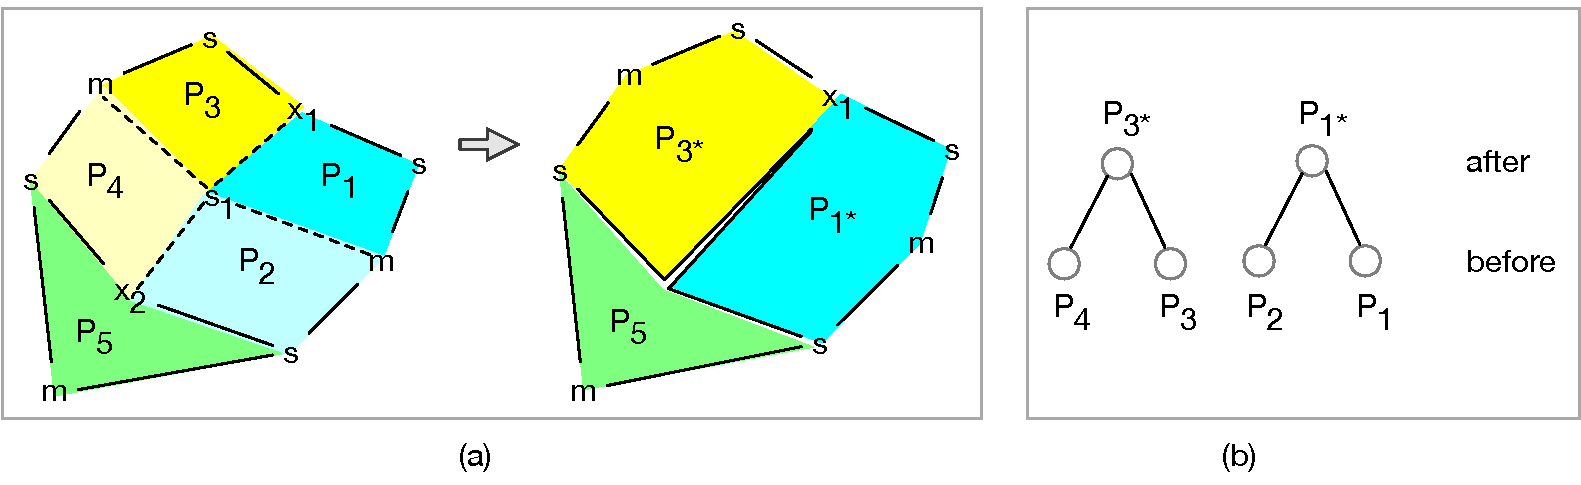
\includegraphics[width=\linewidth]{cancellation}
%     \caption{A simplification step over a 2-manifold: m, x, s represent local minima, maxima and saddles respectively. a) Merging x2 into x1 deletes x2, s1, and the internal edges. In addition, partition P2 merges into P1 and P4 into P3. b) The Regulus perspective represents the single step as two merges of pairs of partitions, forming two nested structures.}
%     \label{fig:cancellation}
%     \end{center}
% \end{figure}

\subsection{Regulus Tree Layout}
\label{sec:tree}
There are dozens of different ways to visualize a tree, yet conceptually all full tree layouts are based on either a top-down or a bottom-up ordering (\autoref{fig:tree-diagram}). The placement of a node is based on the distance of the node from the root (top-down) or a leaf (bottom-up) in terms of the number of parent-child edges. This is true whether the layout is vertical, horizontal, or radial. 
% In addition, tree layouts that employ edges between nodes are not space efficient in the sense that relatively little space is reserved for each node for depicting additional information about the node 

To the best of our knowledge, the \RT layout is new and unique. We describe the new layout in terms of modifying a bottom-up layout. First, we use the vertical axis to depict persistence level \autoref{fig:tree-diagram}c). We then represent a tree node by a rectangle and position it vertically such that its bottom edge is aligned with the persistence level in which it is created. Because the leaves of the tree represent the base partitions, i.e. the partitions of the full \MSC before any simplification, they must, by definition, have a persistence level of 0 and therefore form a single row of rectangles whose bottoms are all aligned. 

When two partitions are merged, the new partition (the parent) must have a persistence level greater than that of its children and thus will be positioned vertically higher than its children. In the horizontal direction, we use the width of the rectangles to encode the number of data points and convey a measure of size. Note that if the data points were sampled uniformly, then the number of points in a partition is roughly proportional to its volume. Since, by definition, a parent contains all the points of its direct children, then the width of the parent is equal to the sum of the widths of its children. Therefore, we can position all the children of a parent sequentially in the horizontal direction without causing overlaps (\autoref{fig:tree-diagram}d). Finally, we extend the top of each node to the base of its parent. The height of a node therefore encodes its lifespan since the base of the parent represents the persistence level the parent is created and the level in which the children are deleted. We note that the vertical axis of the \RT represents persistence and not function value as used in other techniques, such as the contour and merge trees, or the persistence diagram.

\begin{figure}[tb]
    \begin{center}
     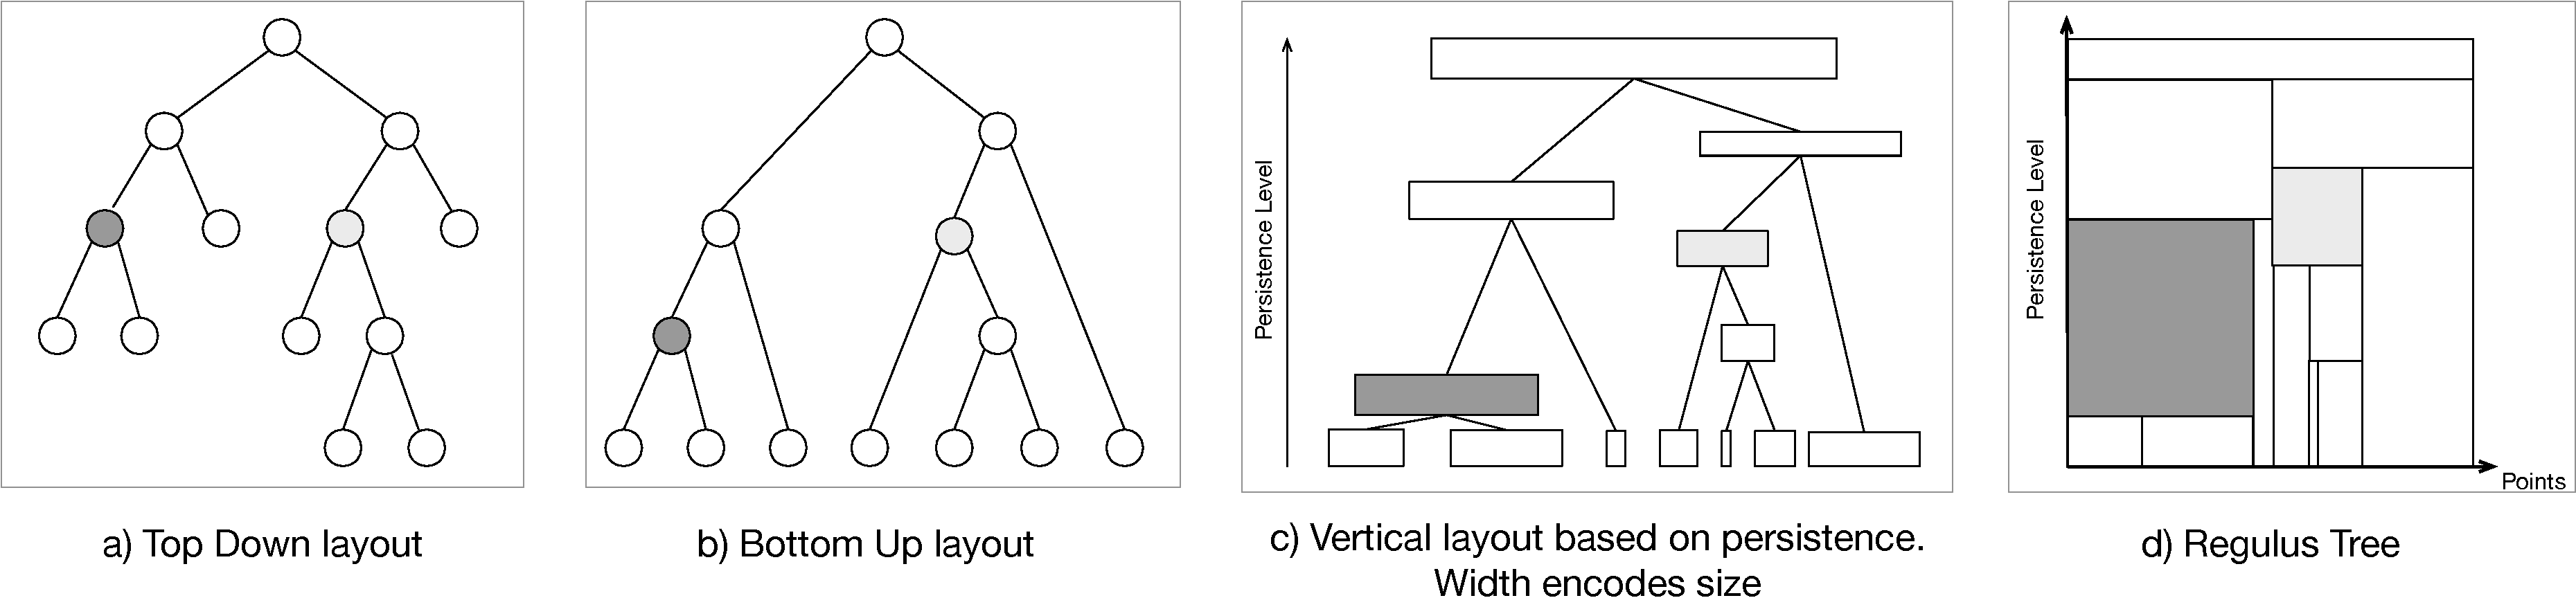
\includegraphics[width=\linewidth]{tree-diagram-1}
    \caption{Typical tree layouts position nodes based on their distance from the top (a) or bottom (b). We use vertical position to encode persistence and width to encode size (c). \RT (d): node height extends to parent to encode lifespan; horizontal layout based on enumeration of the points. Two of the nodes are shaded to illustrate the correspondence between the trees.}
    \label{fig:tree-diagram}
    \end{center}
\end{figure}

We can take advantage of the horizontal layout by enumerating all the data points based on the base partitions they are part of (the enumeration within a partition is not important). Using this approach, we need only two numbers per partition to indicate the range of data points that are contained in that partition. Since the parent partition contains all the data points of its children and the children are positioned sequentially, the partition's data points can also be specified via a range using two numbers. Effectively, we decoupled the data points from the hierarchical structure of the partitions and kept the memory size at $O(n + p)$, where $n$ is the number of data points and $p$ is the number of partitions in the tree.

It is important to note that the above description is correct only with respect to non-critical points, which are shared between partitions. To address this, we initially assign each critical point to one of the base partitions adjacent to it. We then maintain for each partition a short list of all the critical points it's associated with but are not part of its own range of points. In the tree layout, we use the width of a node to encode only the number of points its children contain. This ensures that the parent has the correct visual width to contain all of its children. The exact number of points associated with a partition is provided in a tooltip. This does not pose any problems as the number of extra critical points is minimal. 

\autoref{fig:regulus-tree} shows a \RT associated with a $2d$ scalar function, which we sampled at 2000 points and added small white noise. The horizontal axis represents enumeration of all 2000 points, while the vertical axis represents the relative persistence level in the range of 0 to 1. For illustration purposes we use color to encode the lifespan of each node, i.e the difference between the persistence value of the parent and the persistence value of the node. 

The \RT is \textit{not} a TreeMap despite the superficial similarity. A TreeMap depicts the leaves of a tree using a 2D layout that takes into consideration the tree hierarchy, and the two axes do not have individual meaning. A few variations do incorporate some information about the parents, but because the emphasis is on the leaves, the parents are depicted differently and are mainly used to convey structure. In contrast, the \RT represents the whole tree structure, the two axes have precise and different meaning and for the most part the leaves are the least important features.

\begin{figure}[tb]
    \begin{center}
    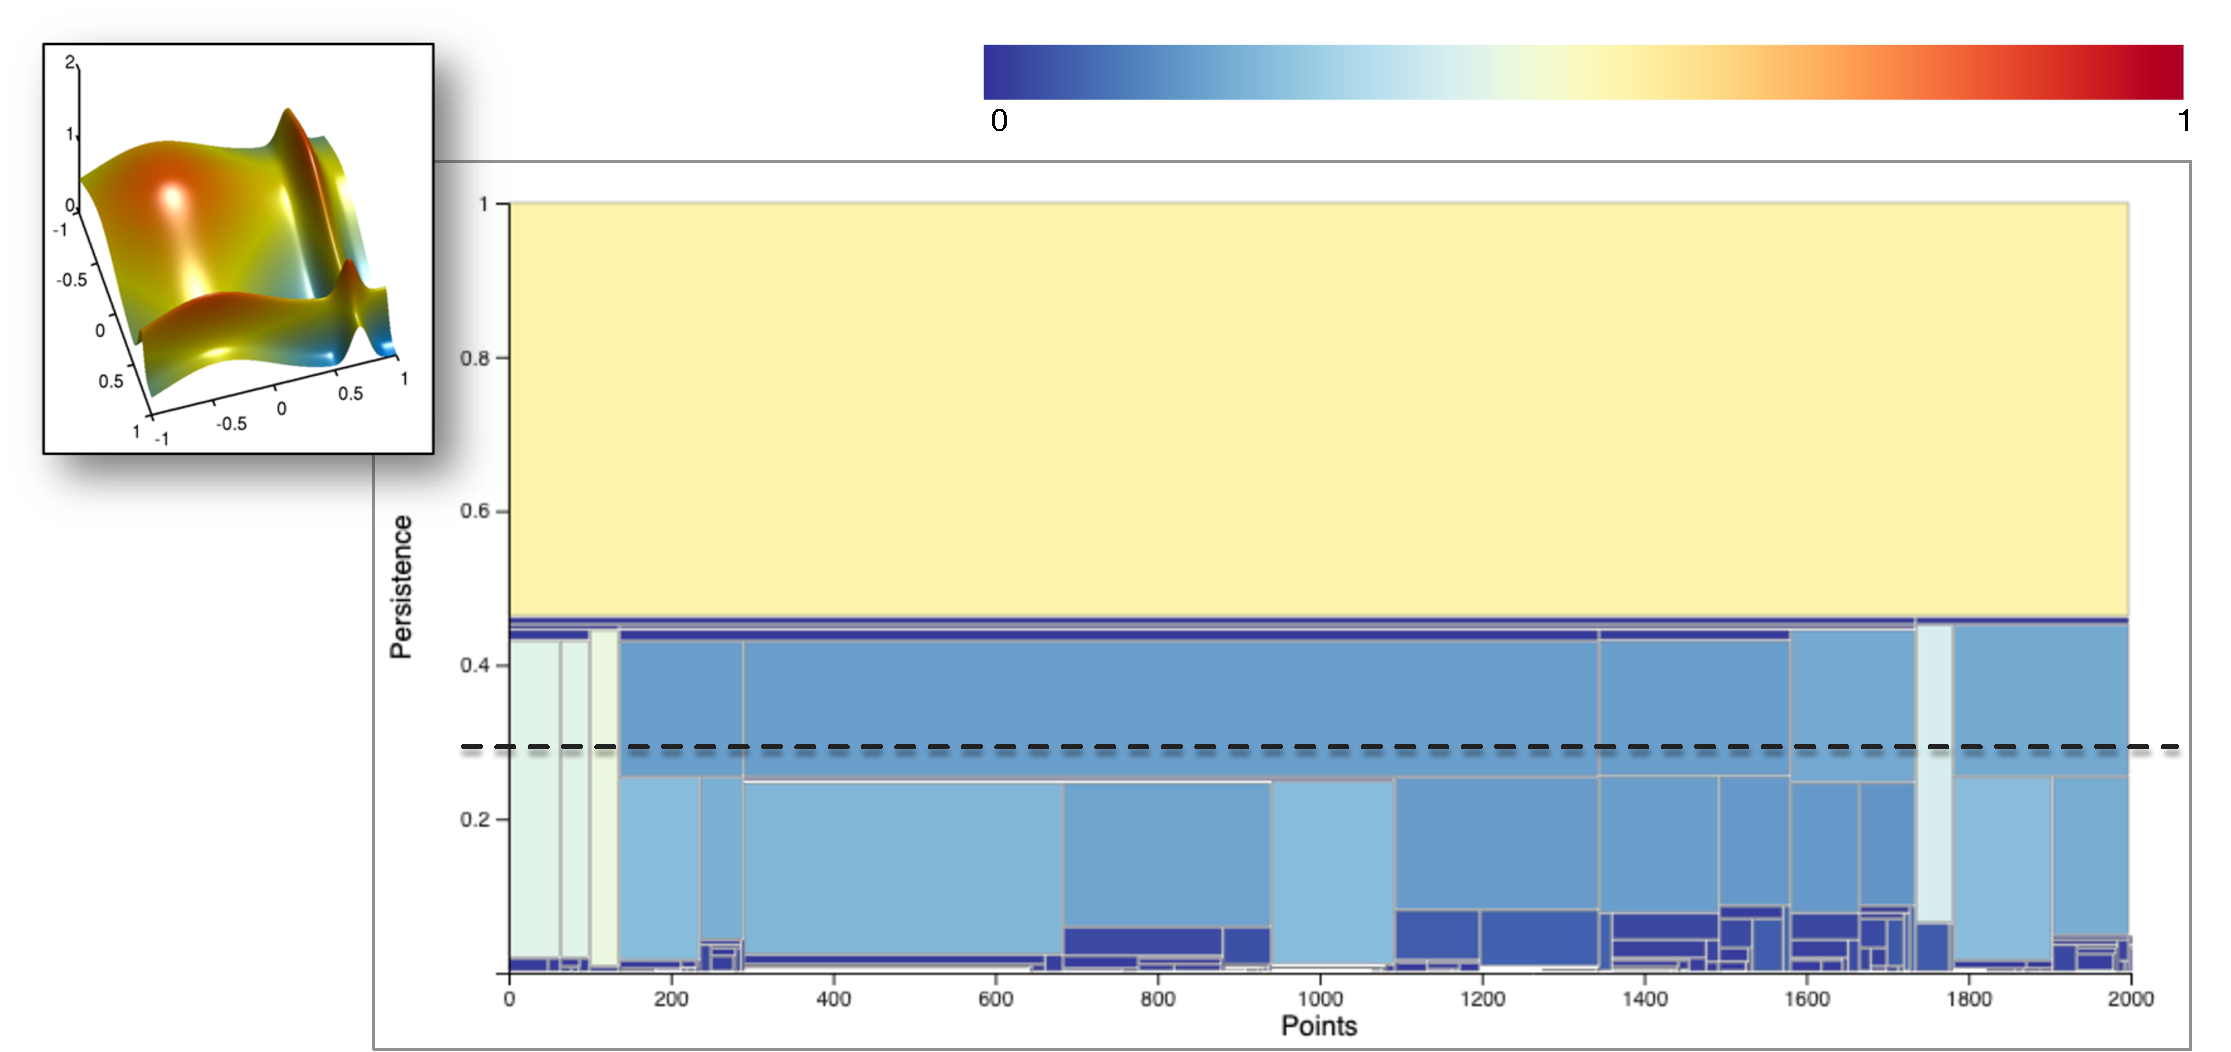
\includegraphics[width=\linewidth]{example}
    \caption{A 2D scalar function and a corresponding \RT. For illustration purpose, color encodes the lifespan of a partition using the blue-yellow-red colormap shown at the top. Selecting persistence level of 0.3 amount to selecting the nodes that intersect the dashed line.}
    \label{fig:regulus-tree}
    \end{center}
\end{figure}

\subsection{Simplifying the Tree}
\label{sec:filtering}
Despite its compactness, the \RT can become quite large for large datasets with complex topology. In addition to pan and zoom, we can also visually simplify the tree without changing the layout by hiding nodes based on some filtering criteria. In both cases only the visualization of the tree is modified but not the tree itself. More often than not, though, we want to simplify the tree itself.

Persistence is often used to help separate between noise and real features by removing features with low persistence level, which amounts to pruning the tree at a certain  threshold. From the technical perspective, persistence provides some measure of the dominance and stability of a critical point, suggesting which features should be preserved. The partition perspective of the \RT offers a different way to think of persistence. Consider the \RT depicted in \autoref{fig:reduce}b and the two narrow green and purple partitions, both of which have a relatively short lifespan but may actually represent a merger of two prominent features. The higher the node is located along the vertical axes, the higher the persistence levels of the two features being merged and the deeper the valley between the two mountains is (or the taller the ridge between two valleys is). 

From the perspective of the Regulus Tree, such partitions are unstable and can be regarded as a relative noise within their local neighborhood. In terms of creating a simplified description of the topology, removing these partitions is akin to depicting a mountain range by only one or two mountains. We  extend this notion of simplifying the topology by simplifying the \RT to also include removing small partitions (thin partitions with few points), partitions with points with values outside a range of interest, and in general filtering the function the user may wish to apply.

While removing small noise amount to pruning the tree, filtering specific nodes does not amount to removing their children. Instead we attach the children to their grandparent  (\autoref{fig:reduce}a), which means that in general a \RT is not a binary tree. We compute a full tree simplification by traversing the tree depth-first and considering one node at a time. If many nodes are removed the new tree may end up with tall and skinny nodes. This is especially the case if we insist on keeping base partitions even if the original lifespan is too small. Our approach is to remove such base partitions and allow the tree to have a jagged edge at the bottom (\autoref{fig:transition}). 
 
We do need to ensure that the new tree represents a valid simplification of the topology. Since a node/partition is the sum of its children, it contains all of their points and thus the grandparent must by definition already contain the points of its new direct children. Another issue to consider is the lifespan of the remaining partitions. We defined the lifespan as the difference between the persistence levels of the parent and the partition. For this reason, we do not store the lifespan of a partition in the partition record; rather, we compute it on the fly based on the parent-child relationship of the node pointing to it. The lifespan of a partition is therefore relative to the tree pointing to it and a partition may have different vertical height (lifespan) after the simplification/transformation of the tree. 

In general, we do not modify the original tree; rather, we create a new tree hierarchy that refers to a shared collection of partitions. In this sense, each tree is a view over the collection of partitions, similar to creating a sub-array as a view of the full array. 
% The separation between the tree structure and the collection of partitions allows us to create multiple trees all pointing to the same set of partitions, although each tree may refer to only some of the partitions. This in turn allow us to visualize multiple trees side by side, representing variation of nested hierarchies, a kind of collection of meta-simplifications of the topology. 

\begin{figure}[tb]
    \begin{center}
     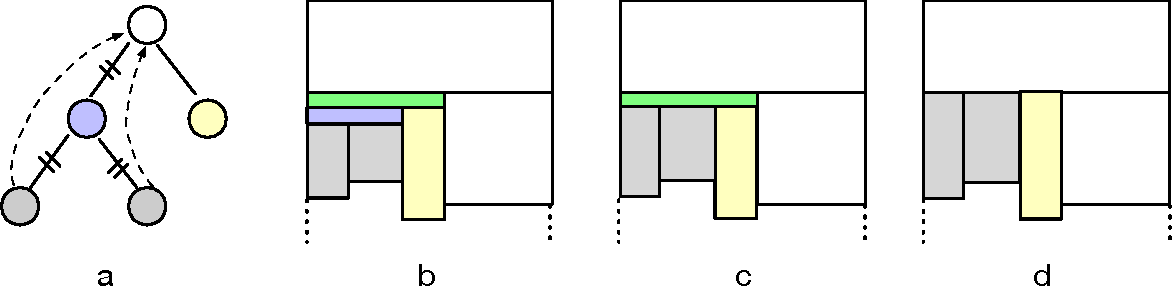
\includegraphics[width=\linewidth]{reduce-2}
    \caption{Simplifying a Regulus Tree by removing intermediate nodes. 
    % The parent node represents multiple half simplification steps (recall that one simplification step leads to multiple partitions merges).
    }
    \label{fig:reduce}
    \end{center}
\end{figure}


\subsection{Exploration and Simplifications Strategies}
\label{sec:simplification}

In addition to providing a concise global overview, the structure of the \RT can be used to help guide the exploration and determine where to simplify, 
\begin{itemize}[label={}, leftmargin=0pt, noitemsep]
    \item  \textit{Global simplification}: In the context of the Regulus Tree, a persistence value maps to a single horizontal line as shown by the red dashed line in \autoref{fig:strategies}a. Since we do not compute level sets, it doesn't matter where the line intersects a partition, only that it does.  While the persistence graph only indicates the number of active critical points for the given persistence value, the \RT provides insights about the size (width) and stability (height) of the partitions. The tree structure may, for example, reveal  that a section of the persistence graph that is not a plateau is actually composed mostly of stable partitions throughout the domain except for instabilities in a small part of the domain or maybe in a number of small partitions that are likely not significant.

    \item  \textit{Adaptive simplification}: Consider a height function depicting the geographic elevation of a valley in a mountainous area. Perturbations that might not be important in the rugged mountains may have significant importance in the flat valley area. We can apply the notion of local simplification in the context of the \RT by selecting a step like line, such a the red line in \autoref{fig:strategies}b. We do not alter the meaning of the simplifications. We only select a subset of the original simplifications. No new partitions are introduced.
    
    The adaptive simplification is easy to understand in the context of the \RT but computing the boundary or interpolating a continuous function across the selected partitions might not be a trivial task as the boundary will include T-junctions. This is not an issue in the context of this work as we focus on understanding the general structure of the underlying function and identify interesting regions.
    
    \item  \textit{Discrete selection}: Supporting a selection based on single persistence value is simple as it requires moving a single horizontal line up and down. The local simplification is more complex and would require interactive construction of a line with potentially multiple steps (adding and removing steps, adjusting step vertical and horizontal positions). A simpler approach is to allows the user to directly select (e.g. click on) the partitions the step line should pass through \autoref{fig:strategies}b.
    
    \item  \textit{Non-continuous selection}: For the purpose of identifying and exploring interesting partitions, it is sufficient to select only partitions of interest (\autoref{fig:strategies}c) to quickly compare and contrast the properties of partitions at different persistence levels. This is by far the most often used selection method we employ in our workflows.
    
    \item \textit{Non-consistent simplification}: We can generalize the non-continuous selection by selecting partitions that overlap horizontally, that is a partition and its descendent (\autoref{fig:strategies}d). There are two reasons for using  non-consistence simplification. One is to simply compare the properties of a partition with its parent to determine if the parent provides sufficient details. The process can be repeated up and down the tree hierarchy if a more fine tune simplification of the whole \MSC is required. The second reason has to do with efficient representation. Consider a quadtree partitioning of a relatively smooth function except for one small area as shown in \autoref{fig:strategies}e. This space decomposition is often critical in many applications, despite the fact that 12 of the 13 partitions are very similar. On the other hand, when studying the structure of the underlying function, a more efficient representation might consist of only two nested regions as shown in \autoref{fig:strategies}f, which provides both a global view and local details.
\end{itemize}

\begin{figure}[tb]
    \begin{center}
    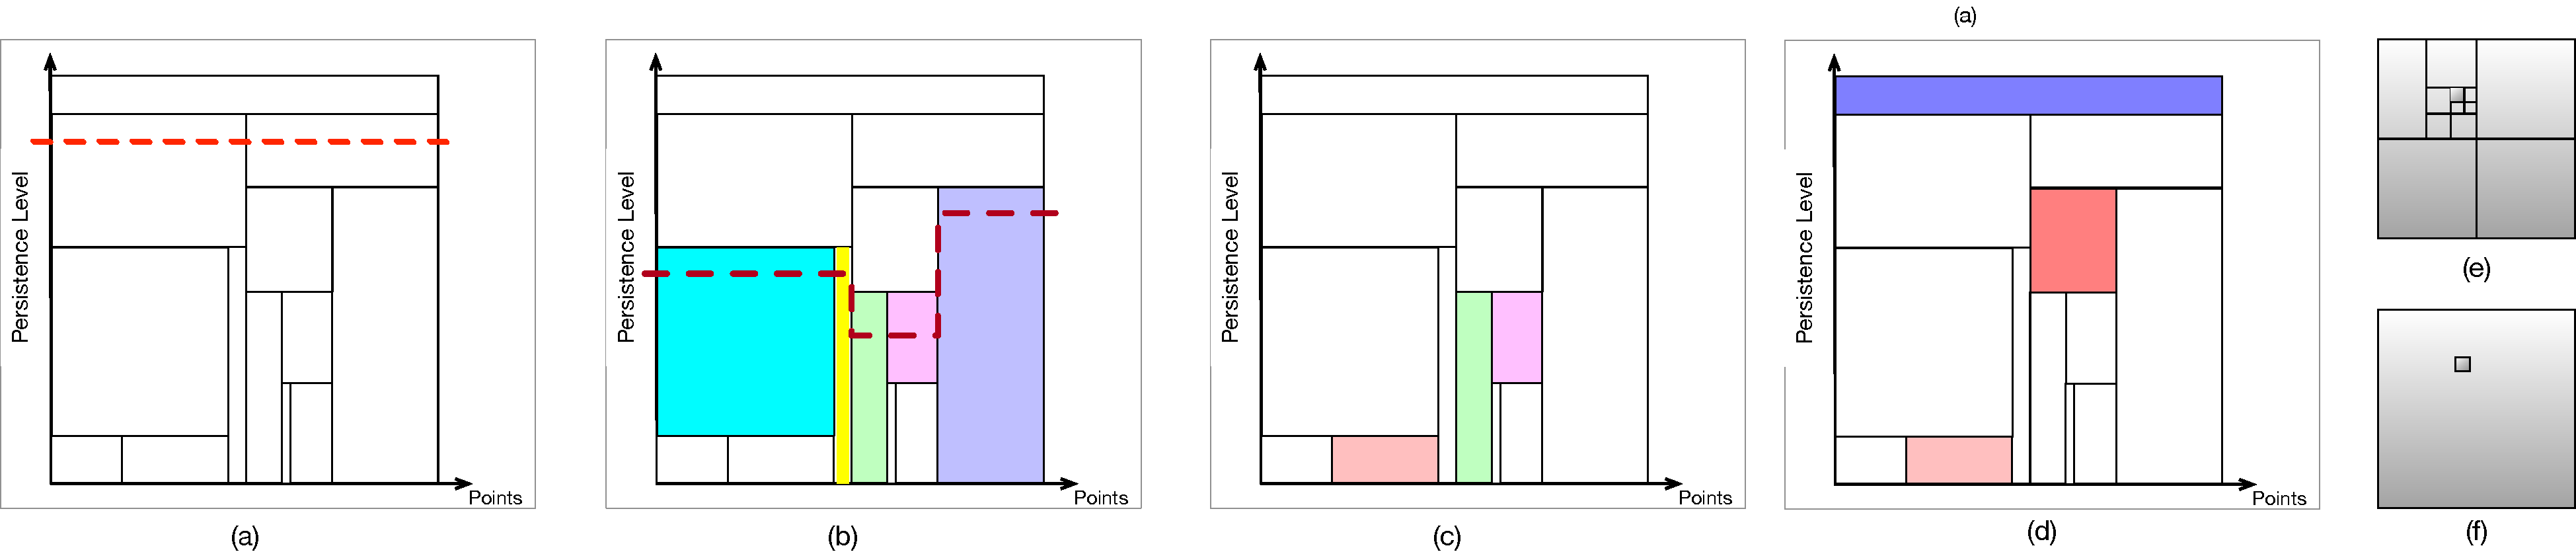
\includegraphics[width=\linewidth]{strategies-4}
    \caption{Exploration strategies. a) global simplification b) adaptive simplification c) non-continuous selection d) non-consistent simplification. e-f) The rational for non-consistent simplification (see text)}
    \label{fig:strategies}
    \end{center}
\end{figure}

 